\newpage
\section{チャレンジ問題(2):GIF アニメーションの作成}
\label{GIF}
gif アニメーションを使ってスライドショー作ってみましょう。gif とは\ruby{画像}{が|ぞう}ファイルのフォーマットの 1 つで、アニメーションを\ruby{表現}{ひょう|げん}することもできます。\\
\begin{enumerate}
\item ディレクトリ slideshow をホームディレクトリに作りましょう。\\
\item スライドショーの\ruby{素材}{そ|ざい}(パラパラ\ruby{漫画}{まん|が}の\ruby{一枚}{いち|まい}一枚)を集めます。インターネットで画像を\ruby{検索}{けん|さく}したり、Gimp で作ったりしましょう。画像は今作った slideshow というディレクトリに\ruby{保存}{ほ|ぞん}しましょう。\\
\item 画像の名前が連番になるように名前を\ruby{変更}{へん|こう}します。00.jpg 01.jpg 02.jpg … のようにスライドショーで\ruby{表示}{ひょう|じ}したい順番の番号を名前にしましょう。\\
\begin{figure}[H]
    \centering
    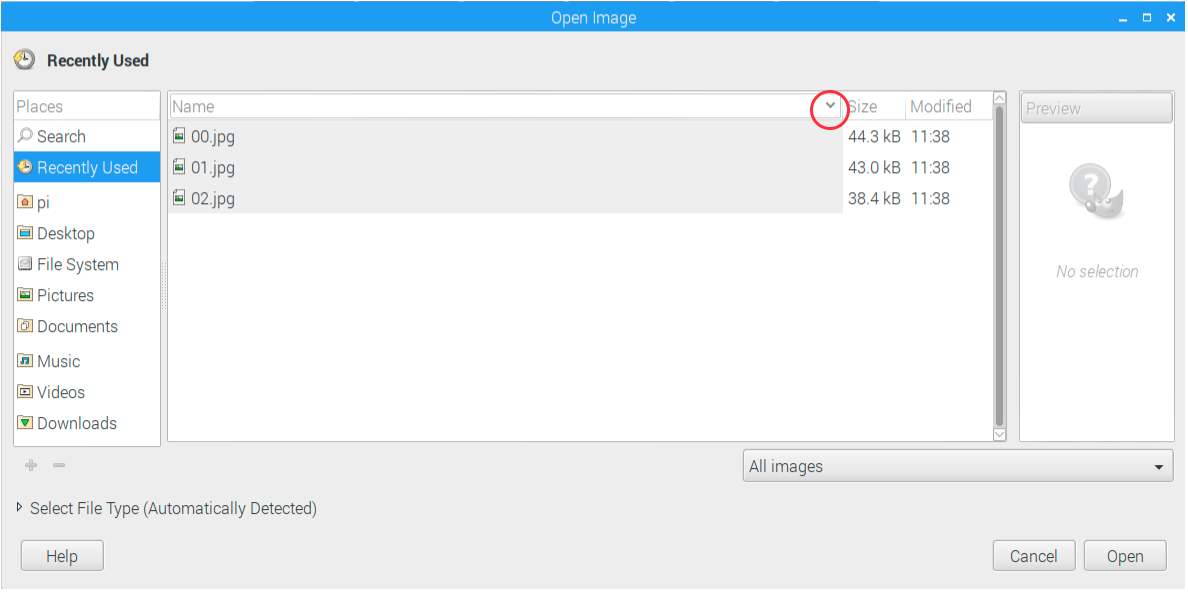
\includegraphics[width=\linewidth]{images/chap03/text03-img025.png}
\end{figure}
\item Gimp を開きます。「ファイル」→「開く/インポート」で「画像ファイルを開く」ウィンドウを出し、最初の一枚目を\ruby{選択}{せん|たく}して開きます。Gimp で「ファイル」→「レイヤーとして開く」で、2 番め\ruby{以降}{い|こう}の全てのファイルを選択して開きましょう。Shift キーを\ruby{押}{お}しながらクリックすることで\ruby{複数}{ふく|すう}選択できます。選択するときは、「名前」をクリックして名前の順に\ruby{並}{なら}び\ruby{替}{か}えておきましょう。\\
\item Gimp で「ファイル」→「名前をつけてエクスポート」をクリックします。名前をslideshow.gif とし、エクスポートボタンを押します。
\begin{figure}[H]
    \centering
    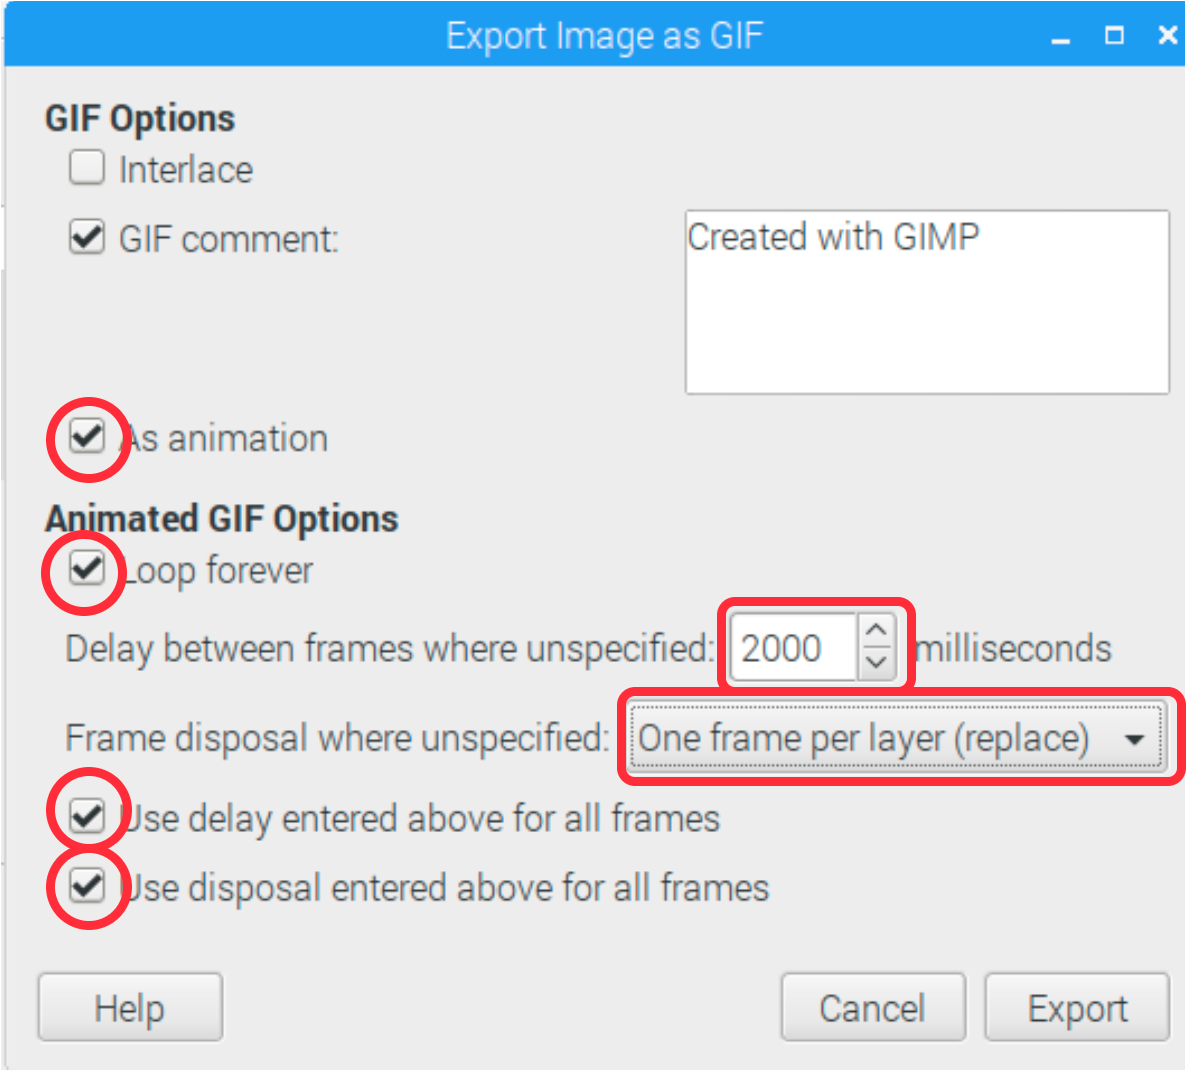
\includegraphics[width=0.6\linewidth]{images/chap03/text03-img026.png}
\end{figure}
\item 「画像をエクスポート: GIF 形式」というウィンドウが出るので、「アニメーションとしてエクスポート」にチェック、「指定しない場合のディレイ」をお好みに(2000 ミリ秒くらいがオススメ)、「指定しない場合のフレーム処理」を「レイヤーごとに 1 フレーム(\ruby{置換}{ち|かん})」に、「全フレームのディレイにこの\ruby{値}{あたい}を使用」にチェック、「全フレームのフレーム処理にこの値を使用」にチェックをしてエクスポートボタンを押します。\\
\item 出来上がった画像をみてみましょう。下記どちらかのコマンドでみることができます。\\
chromium-browser slideshow/slideshow.gif\\
eom slideshow/slideshow.gif\\
cd コマンドなどでフォルダを移動した場合は、cd コマンドでホームディレクトリに移動してから上記のコマンドを入力しましょう。
\end{enumerate}

\begin{tcolorbox}[title=\useOmetoi]
%\begin{minipage}{0.94\hsize}
\begin{enumerate}
\addex{\ref{GIF}を見ながら、オリジナルのアニメーションを作成しましょう。カメラで何枚か画像をさつえいします。カメラを動かさずに、写す物を少しずつ動かしながらさつえいします。さつえいと、物を少し動かすことを\ruby{繰}{く}り返すと、アニメーションを作ることができます。}
\end{enumerate}
%\end{minipage}
\end{tcolorbox}
